\documentclass[table]{beamer}
\usetheme{gpmeet}
\graphicspath{{../../figures/}}

\newcommand{\leftRect}[2]{\node[draw=text,very thick,rounded corners, text width=0.46\textwidth,minimum height=6cm] at (0,0) {\centering\textbf{#1}\\ \raggedright \color{text}#2};}
\newcommand{\rightRect}[2]{\node[draw=text,very thick,rounded corners, text width=0.46\textwidth,minimum height=6cm] at (0.54\textwidth,0) {\centering\textbf{#1}\\ \raggedright \color{text}#2};}

\usepackage{tikz}

\title{Group meetings}

\subtitle{Memristors-based recurent modules for neural computing}

\author[V. BARBAZA]{Valentin BARBAZA}

\date{05/06/2023}

\logo{
  \begin{tikzpicture}[overlay,remember picture]
    \node[below=1pt] at (current page.55){
      
\includegraphics[height=1cm]{logos/ist}
      \hspace{1pt}
      
\includegraphics[height=1cm]{logos/inesc-mn.png}
      
\includegraphics[height=1cm]{logos/inesc-id.eps}
    };
  \end{tikzpicture}
  }

  \begin{document}

  \frame{\titlepage}


  \begin{frame}
    \frametitle{Introduction}

    \begin{itemize}
        \color{text}
      \item I am working on an analog implementation of a LSTM Neural Networks.
      \item The final objective of my thesis is to have a successful simulation of such a circuit.
    \end{itemize}

  \end{frame}


  \begin{frame}
    \frametitle{Introduction}
    \centering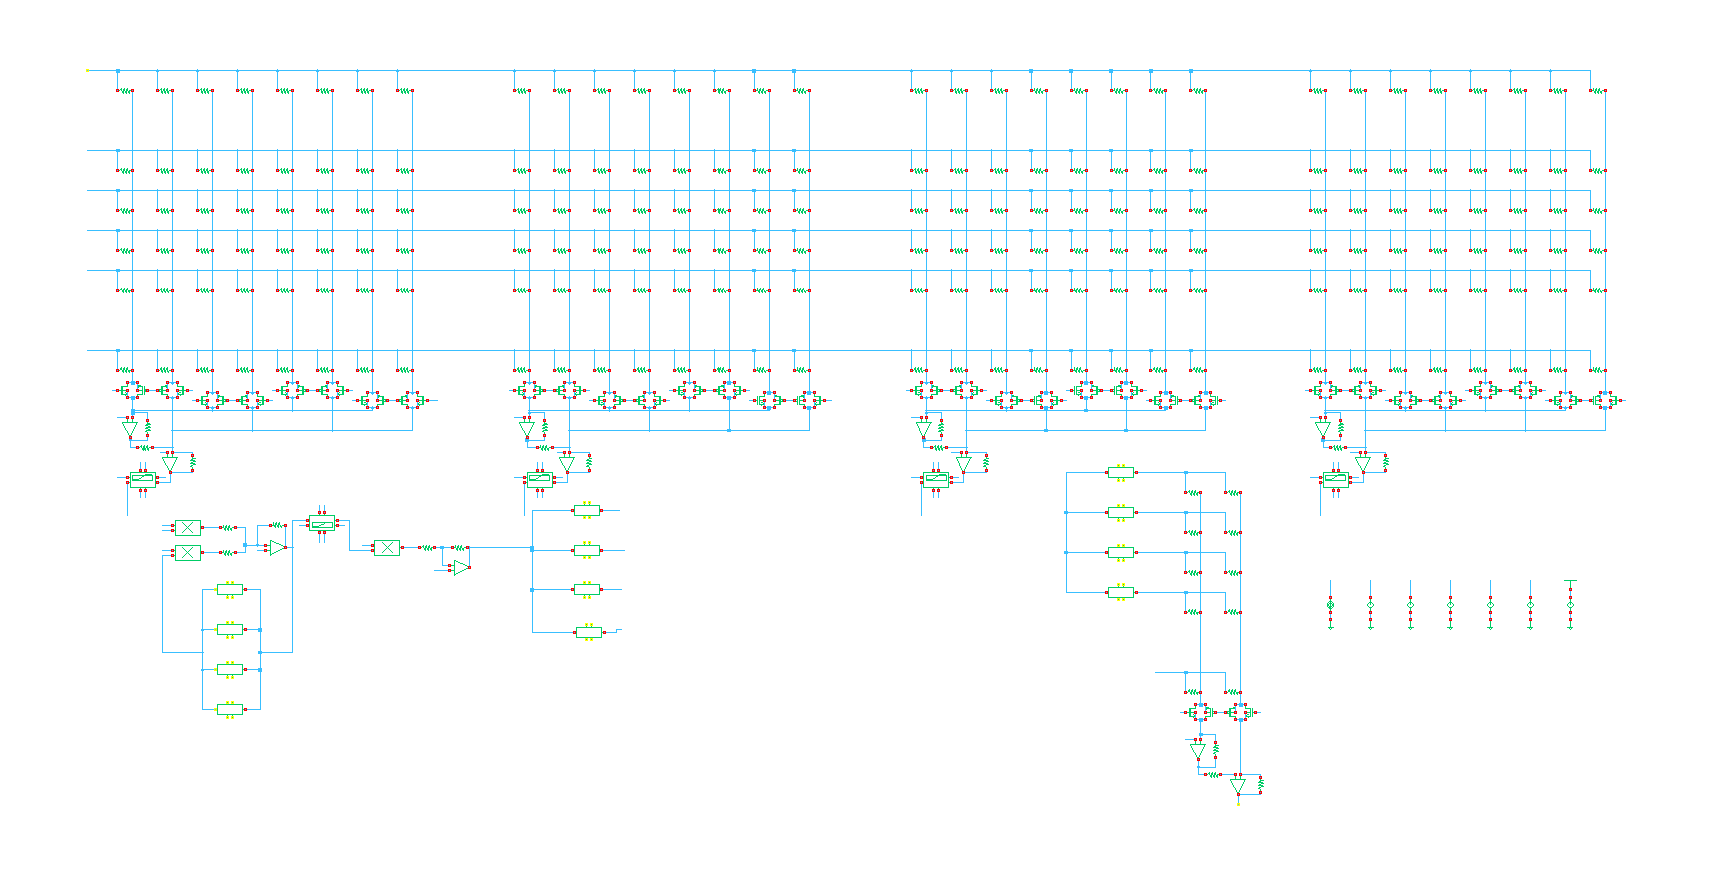
\includegraphics[width=\textwidth]{lstm/lstm-np}
  \end{frame}

  \begin{frame}
    \frametitle{Last weeks...}

    Last meeting, I promised to do :

    \centering
    \rowcolors{2}{evenRow}{oddRow}
    \begin{tabular}{ c m{3cm} c m{3cm} c }
      \rowcolor{firstRow}
      \color{white}\textbf{\#} & \centering\color{white}Task & \color{white}Done? & \color{white}Why not? & \color{white}Help? \\
      1 & Try to use LTSpice & No & Found out I could do what I want with Cadence & No\\
      2 & Find another\newline problem to work on & No & Lack of time & Yes\\
      3 & Work on the thesis intro & on going &  & No\\
    \end{tabular}

  \end{frame}

  \begin{frame}{What's new}
    \begin{itemize}
      \item Results obtianed :
        \begin{itemize}
            \color{text}
          \item With the help of Fabio, I can now simulate all the steps automatically
          \item I successfully ran the simulation
          \item The result are not correct
        \end{itemize}
      \item Improvements :
        \begin{itemize}
            \color{text}
          \item Debug the whole thing
        \end{itemize}
    \end{itemize}
  \end{frame}

  \begin{frame}{What's new}
    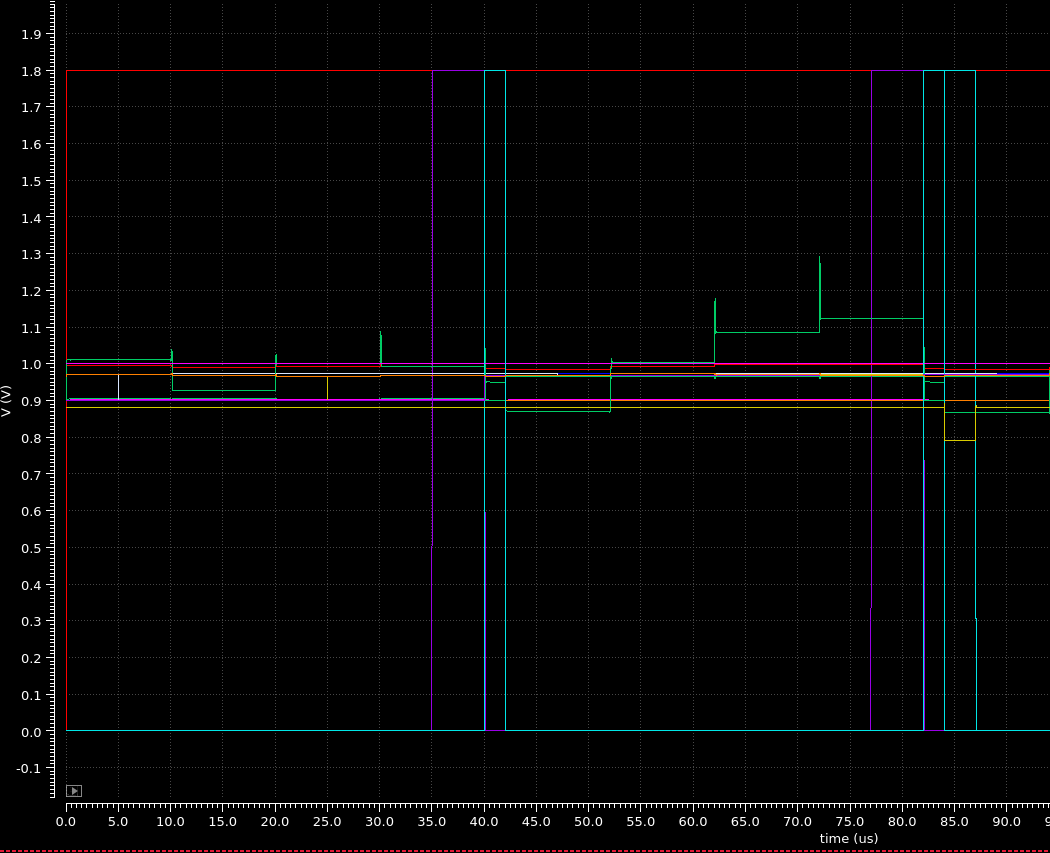
\includegraphics[width=\textwidth]{fulltrial1/fulltrial1-all-curves}
  \end{frame}

  \begin{frame}<1>[label=prob]
    \frametitle{Problems/doubts}
    \begin{itemize}
      \item<1-> The memory doesn't output the right values
      \item<2-> The memory input seems to be active for too long
      \item<3-> The output of the sigmoid doesn't look right
      \item<4-> The output result isn't what is expected
    \end{itemize}
  \end{frame}

  \begin{frame}{Problems/doubts}
    The memory doesn't output the right values.

    \centering
    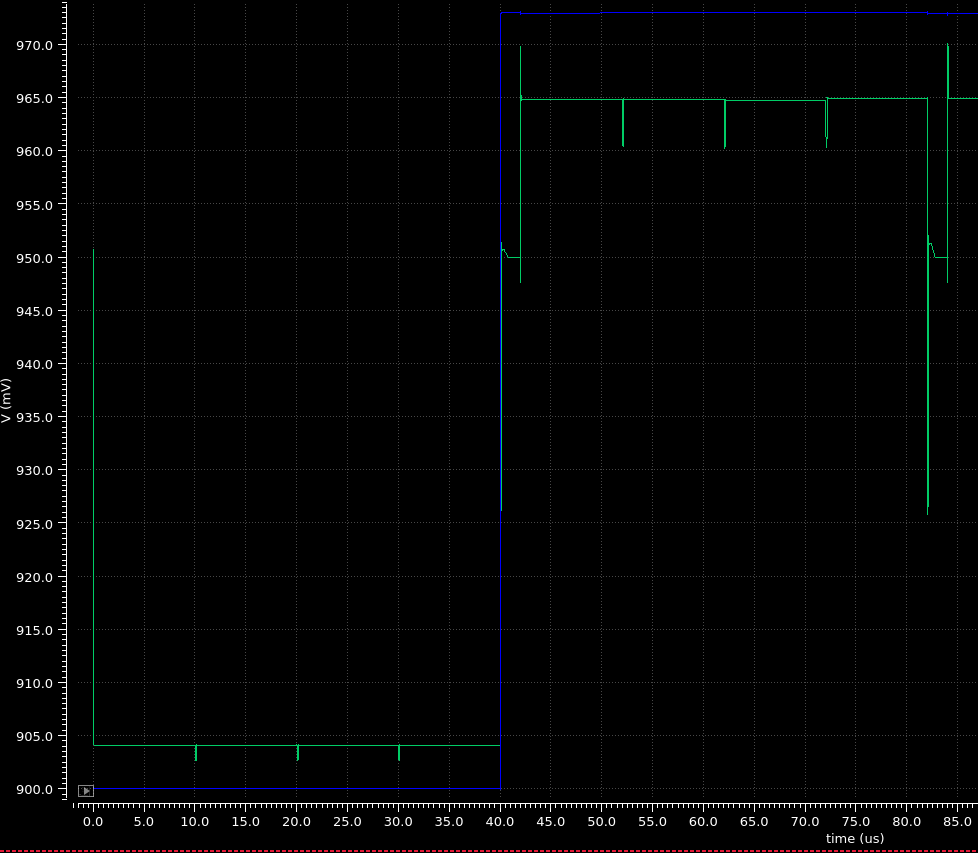
\includegraphics[width=0.7\textwidth]{fulltrial1/fulltrial1-memory-prob}
  \end{frame}

  \againframe<2>{prob}

  \begin{frame}{Problems/doubts}
    \centering
    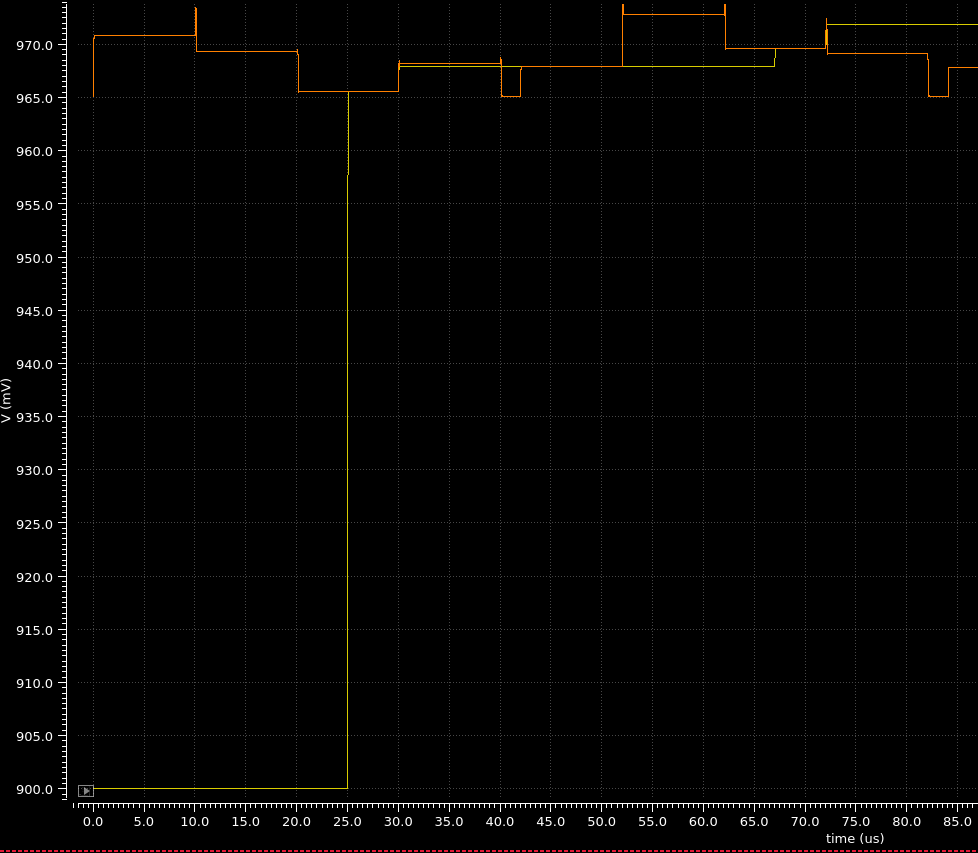
\includegraphics[width=1\textwidth]{fulltrial1/fulltrial1-mem-act-late}
  \end{frame}

  \againframe<3>{prob}
  \begin{frame}{Problems/doubts}
    \begin{figure}[!tbp]
      \centering
      \begin{minipage}[b]{0.4\textwidth}
        \centering
        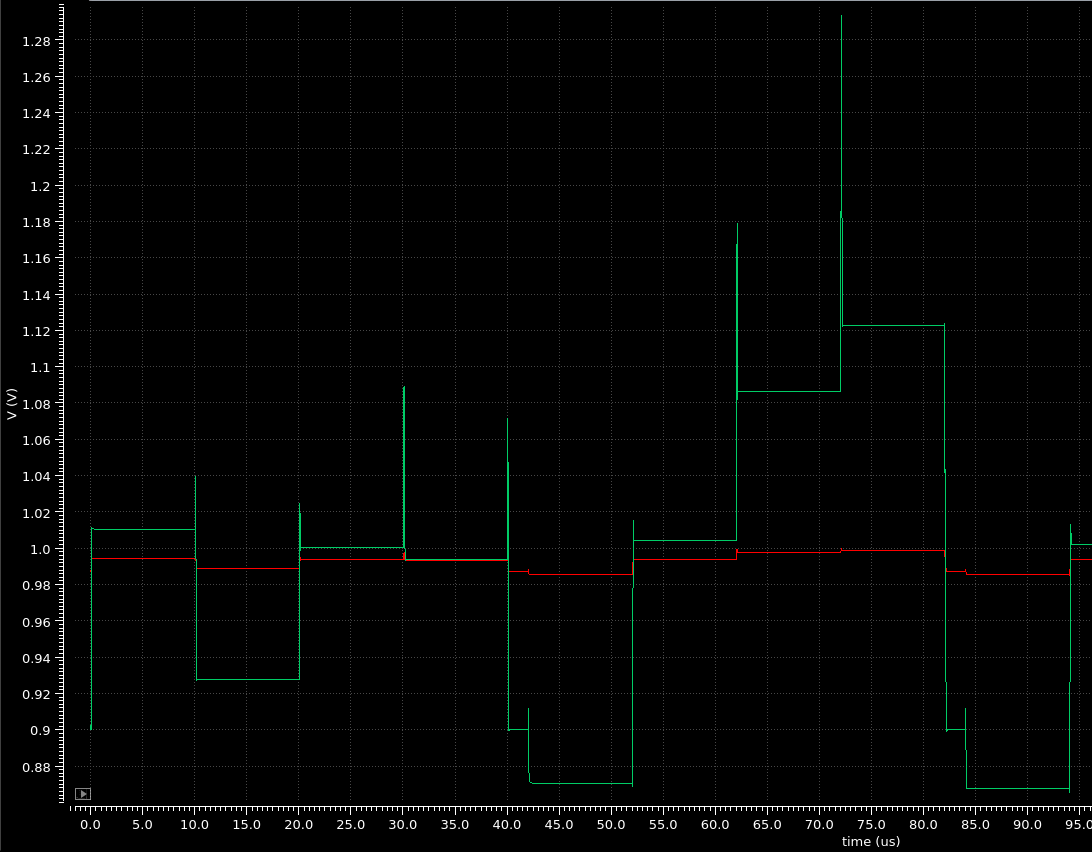
\includegraphics[width=\textwidth]{fulltrial1/sigmoid-prob.png}
      \end{minipage}
      \hspace{20pt}
      \begin{minipage}[b]{0.4\textwidth}
        \centering
        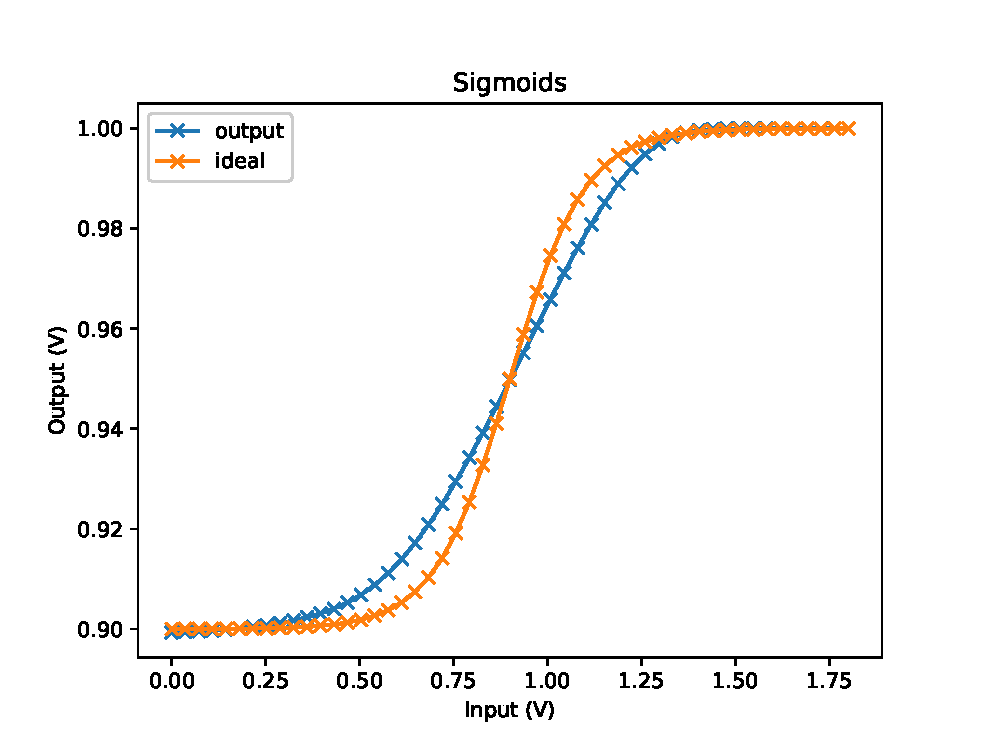
\includegraphics[width=\textwidth]{activation/sigmoid}
      \end{minipage}
    \end{figure}
  \end{frame}

  \againframe<4>{prob}
  \begin{frame}{Problems/doubts}
    The output is ~0.791 V. This is $-1.09$ and should be $0.015$

    \centering
    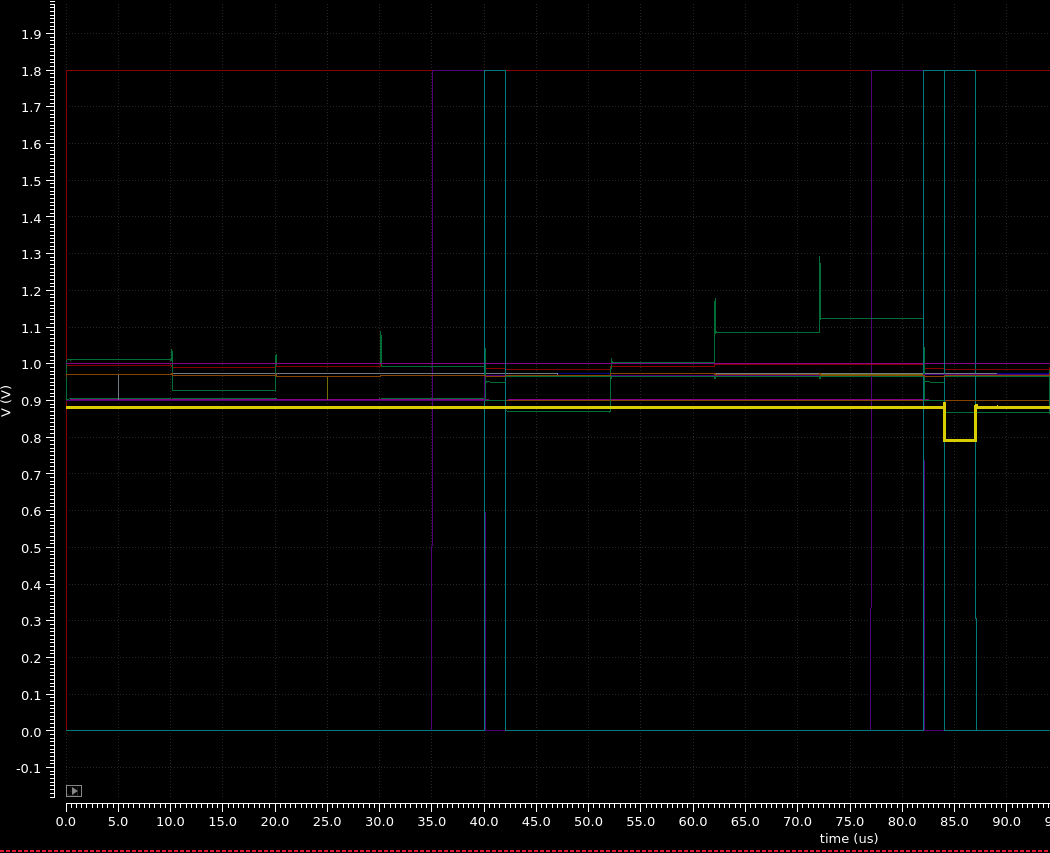
\includegraphics[width=\textwidth]{fulltrial1/fulltrial1-final-res}
  \end{frame}


  \begin{frame}{Next weeks}

    List of what I plan to do in the next weeks :

    \centering
    \rowcolors{2}{evenRow}{oddRow}
    \begin{tabular}{ c m{4cm} }
      \rowcolor{firstRow}
      \color{white}\textbf{\#} & \centering\color{white}Task \cr
      1 & Find another LSTM problem \\
      2 & "Debug" the circuit \\
      2.1 & Run the entire simulation \\
      3 & Work on thesis \\
    \end{tabular}
  \end{frame}

  \begin{frame}{Networking and sharing}
    \begin{tikzpicture}
      \leftRect{Help/Collaboration :}{- If anybody has any idea of an interesting LSTM/NN problem to work on.\\-Also if any phenomen happening are familiar to you, I'll take the help}

      \rightRect{Recommendations :}{I worked on a latex/beamer version of the template}
    \end{tikzpicture}
  \end{frame}

\end{document}
